\batchmode
\documentclass[twoside]{book}

% Packages required by doxygen
\usepackage{fixltx2e}
\usepackage{calc}
\usepackage{doxygen}
\usepackage[export]{adjustbox} % also loads graphicx
\usepackage{graphicx}
\usepackage[utf8]{inputenc}
\usepackage{makeidx}
\usepackage{multicol}
\usepackage{multirow}
\PassOptionsToPackage{warn}{textcomp}
\usepackage{textcomp}
\usepackage[nointegrals]{wasysym}
\usepackage[table]{xcolor}

% Font selection
\usepackage[T1]{fontenc}
\usepackage[scaled=.90]{helvet}
\usepackage{courier}
\usepackage{amssymb}
\usepackage{sectsty}
\renewcommand{\familydefault}{\sfdefault}
\allsectionsfont{%
  \fontseries{bc}\selectfont%
  \color{darkgray}%
}
\renewcommand{\DoxyLabelFont}{%
  \fontseries{bc}\selectfont%
  \color{darkgray}%
}
\newcommand{\+}{\discretionary{\mbox{\scriptsize$\hookleftarrow$}}{}{}}

% Page & text layout
\usepackage{geometry}
\geometry{%
  a4paper,%
  top=2.5cm,%
  bottom=2.5cm,%
  left=2.5cm,%
  right=2.5cm%
}
\tolerance=750
\hfuzz=15pt
\hbadness=750
\setlength{\emergencystretch}{15pt}
\setlength{\parindent}{0cm}
\setlength{\parskip}{3ex plus 2ex minus 2ex}
\makeatletter
\renewcommand{\paragraph}{%
  \@startsection{paragraph}{4}{0ex}{-1.0ex}{1.0ex}{%
    \normalfont\normalsize\bfseries\SS@parafont%
  }%
}
\renewcommand{\subparagraph}{%
  \@startsection{subparagraph}{5}{0ex}{-1.0ex}{1.0ex}{%
    \normalfont\normalsize\bfseries\SS@subparafont%
  }%
}
\makeatother

% Headers & footers
\usepackage{fancyhdr}
\pagestyle{fancyplain}
\fancyhead[LE]{\fancyplain{}{\bfseries\thepage}}
\fancyhead[CE]{\fancyplain{}{}}
\fancyhead[RE]{\fancyplain{}{\bfseries\leftmark}}
\fancyhead[LO]{\fancyplain{}{\bfseries\rightmark}}
\fancyhead[CO]{\fancyplain{}{}}
\fancyhead[RO]{\fancyplain{}{\bfseries\thepage}}
\fancyfoot[LE]{\fancyplain{}{}}
\fancyfoot[CE]{\fancyplain{}{}}
\fancyfoot[RE]{\fancyplain{}{\bfseries\scriptsize Generated by Doxygen }}
\fancyfoot[LO]{\fancyplain{}{\bfseries\scriptsize Generated by Doxygen }}
\fancyfoot[CO]{\fancyplain{}{}}
\fancyfoot[RO]{\fancyplain{}{}}
\renewcommand{\footrulewidth}{0.4pt}
\renewcommand{\chaptermark}[1]{%
  \markboth{#1}{}%
}
\renewcommand{\sectionmark}[1]{%
  \markright{\thesection\ #1}%
}

% Indices & bibliography
\usepackage{natbib}
\usepackage[titles]{tocloft}
\setcounter{tocdepth}{3}
\setcounter{secnumdepth}{5}
\makeindex

% Hyperlinks (required, but should be loaded last)
\usepackage{ifpdf}
\ifpdf
  \usepackage[pdftex,pagebackref=true]{hyperref}
\else
  \usepackage[ps2pdf,pagebackref=true]{hyperref}
\fi
\hypersetup{%
  colorlinks=true,%
  linkcolor=blue,%
  citecolor=blue,%
  unicode%
}

% Custom commands
\newcommand{\clearemptydoublepage}{%
  \newpage{\pagestyle{empty}\cleardoublepage}%
}

\usepackage{caption}
\captionsetup{labelsep=space,justification=centering,font={bf},singlelinecheck=off,skip=4pt,position=top}

%===== C O N T E N T S =====

\begin{document}

% Titlepage & ToC
\hypersetup{pageanchor=false,
             bookmarksnumbered=true,
             pdfencoding=unicode
            }
\pagenumbering{alph}
\pagenumbering{arabic}
\hypersetup{pageanchor=true}

%--- Begin generated contents ---
\chapter{Demo problem\+: Relaxation oscillations of an interface between two viscous fluids}
\label{index}\hypertarget{index}{}\hypertarget{index_q}{}\section{A few quick questions...}\label{index_q}
Since {\ttfamily oomph-\/lib} is developed as open-\/source software, any evidence that the code is being downloaded and used is very helpful for us as it helps to justify our continued work on this project.

We would therefore be extremely grateful if you could provide the information requested in the form below. Pressing the \char`\"{}submit\char`\"{} button will get you to the actual download page.

{\bfseries Note\+:} 
\begin{DoxyItemize}
\item All information will be treated as confidential. 
\item If you provide your email address and check the appropriate box we will add you to our mailing list to inform you of upgrades and bug fixes to the code. Rest assured that the mailing list is {\bfseries very low volume} -- we have better things to do than to bombard you with email. 
\item If you still feel reluctant to provide any of the information requested, feel free to enter some dummy input. The form will check that {\bfseries some} information has been entered but entering your name as \char`\"{}\+Joe Cool\char`\"{} is perfectly acceptable -- this is to discourage people from not providing the information simply because they are too lazy to type... 
\end{DoxyItemize}



 







 

 \hypertarget{index_pdf}{}\section{P\+D\+F file}\label{index_pdf}
A \href{../latex/refman.pdf}{\tt pdf version} of this document is available. \end{document}

\chapter{Namespace Index}
\section{Namespace List}
Here is a list of all namespaces with brief descriptions\+:\begin{DoxyCompactList}
\item\contentsline{section}{\hyperlink{namespaceGlobal__Physical__Variables}{Global\+\_\+\+Physical\+\_\+\+Variables} \\*Global variables that represent physical properties }{\pageref{namespaceGlobal__Physical__Variables}}{}
\item\contentsline{section}{\hyperlink{namespaceoomph}{oomph} }{\pageref{namespaceoomph}}{}
\item\contentsline{section}{\hyperlink{namespacePhysical__Variables}{Physical\+\_\+\+Variables} \\*Namespace for the solution of 2D linear shell equation }{\pageref{namespacePhysical__Variables}}{}
\end{DoxyCompactList}

\chapter{Hierarchical Index}
\section{Class Hierarchy}
This inheritance list is sorted roughly, but not completely, alphabetically\+:\begin{DoxyCompactList}
\item Problem\begin{DoxyCompactList}
\item \contentsline{section}{Unstructured\+Solid\+Problem$<$ E\+L\+E\+M\+E\+NT $>$}{\pageref{classUnstructuredSolidProblem}}{}
\end{DoxyCompactList}
\end{DoxyCompactList}

\chapter{Class Index}
\section{Class List}
Here are the classes, structs, unions and interfaces with brief descriptions\+:\begin{DoxyCompactList}
\item\contentsline{section}{\hyperlink{classPMLProblem}{P\+M\+L\+Problem$<$ E\+L\+E\+M\+E\+N\+T $>$} }{\pageref{classPMLProblem}}{}
\item\contentsline{section}{\hyperlink{classGlobalParameters_1_1TestPMLMapping}{Global\+Parameters\+::\+Test\+P\+M\+L\+Mapping} }{\pageref{classGlobalParameters_1_1TestPMLMapping}}{}
\end{DoxyCompactList}

\chapter{File Index}
\section{File List}
Here is a list of all files with brief descriptions\+:\begin{DoxyCompactList}
\item\contentsline{section}{\hyperlink{jeffery__orbit_8cc}{jeffery\+\_\+orbit.\+cc} }{\pageref{jeffery__orbit_8cc}}{}
\item\contentsline{section}{\hyperlink{jeffery__orbit_8txt__doxygenified_8h}{jeffery\+\_\+orbit.\+txt\+\_\+doxygenified.\+h} }{\pageref{jeffery__orbit_8txt__doxygenified_8h}}{}
\item\contentsline{section}{\hyperlink{my__taylor__hood__elements_8h}{my\+\_\+taylor\+\_\+hood\+\_\+elements.\+h} }{\pageref{my__taylor__hood__elements_8h}}{}
\end{DoxyCompactList}

\chapter{Namespace Documentation}
\hypertarget{namespaceGlobal__Physical__Variables}{}\section{Global\+\_\+\+Physical\+\_\+\+Variables Namespace Reference}
\label{namespaceGlobal__Physical__Variables}\index{Global\+\_\+\+Physical\+\_\+\+Variables@{Global\+\_\+\+Physical\+\_\+\+Variables}}


Namespace for physical parameters.  


\subsection*{Functions}
\begin{DoxyCompactItemize}
\item 
Vector$<$ double $>$ \hyperlink{namespaceGlobal__Physical__Variables_afae321364975eb56688ad13abc8ed6b7}{Gravity} (2)
\begin{DoxyCompactList}\small\item\em Gravity vector. \end{DoxyCompactList}\item 
void \hyperlink{namespaceGlobal__Physical__Variables_a87da705b8a46bed337cf5dbdd788b87b}{body\+\_\+force} (const double \&time, const Vector$<$ double $>$ \&x, Vector$<$ double $>$ \&result)
\begin{DoxyCompactList}\small\item\em Functional body force. \end{DoxyCompactList}\item 
void \hyperlink{namespaceGlobal__Physical__Variables_a9780d615ae07c4e00a436ab2973b54e6}{zero\+\_\+body\+\_\+force} (const double \&time, const Vector$<$ double $>$ \&x, Vector$<$ double $>$ \&result)
\begin{DoxyCompactList}\small\item\em Zero functional body force. \end{DoxyCompactList}\end{DoxyCompactItemize}
\subsection*{Variables}
\begin{DoxyCompactItemize}
\item 
double \hyperlink{namespaceGlobal__Physical__Variables_ab814e627d2eb5bc50318879d19ab16b9}{Re} =100
\begin{DoxyCompactList}\small\item\em Reynolds number. \end{DoxyCompactList}\item 
double \hyperlink{namespaceGlobal__Physical__Variables_ab1a845a672b4d74b304639a976dc65c6}{Re\+\_\+inv\+Fr} =100
\begin{DoxyCompactList}\small\item\em Reynolds/\+Froude number. \end{DoxyCompactList}\end{DoxyCompactItemize}


\subsection{Detailed Description}
Namespace for physical parameters. 

\subsection{Function Documentation}
\mbox{\Hypertarget{namespaceGlobal__Physical__Variables_a87da705b8a46bed337cf5dbdd788b87b}\label{namespaceGlobal__Physical__Variables_a87da705b8a46bed337cf5dbdd788b87b}} 
\index{Global\+\_\+\+Physical\+\_\+\+Variables@{Global\+\_\+\+Physical\+\_\+\+Variables}!body\+\_\+force@{body\+\_\+force}}
\index{body\+\_\+force@{body\+\_\+force}!Global\+\_\+\+Physical\+\_\+\+Variables@{Global\+\_\+\+Physical\+\_\+\+Variables}}
\subsubsection{\texorpdfstring{body\+\_\+force()}{body\_force()}}
{\footnotesize\ttfamily void Global\+\_\+\+Physical\+\_\+\+Variables\+::body\+\_\+force (\begin{DoxyParamCaption}\item[{const double \&}]{time,  }\item[{const Vector$<$ double $>$ \&}]{x,  }\item[{Vector$<$ double $>$ \&}]{result }\end{DoxyParamCaption})}



Functional body force. 



Definition at line 62 of file circular\+\_\+driven\+\_\+cavity.\+cc.



References Re\+\_\+inv\+Fr.



Referenced by main().

\mbox{\Hypertarget{namespaceGlobal__Physical__Variables_afae321364975eb56688ad13abc8ed6b7}\label{namespaceGlobal__Physical__Variables_afae321364975eb56688ad13abc8ed6b7}} 
\index{Global\+\_\+\+Physical\+\_\+\+Variables@{Global\+\_\+\+Physical\+\_\+\+Variables}!Gravity@{Gravity}}
\index{Gravity@{Gravity}!Global\+\_\+\+Physical\+\_\+\+Variables@{Global\+\_\+\+Physical\+\_\+\+Variables}}
\subsubsection{\texorpdfstring{Gravity()}{Gravity()}}
{\footnotesize\ttfamily Vector$<$double$>$ Global\+\_\+\+Physical\+\_\+\+Variables\+::\+Gravity (\begin{DoxyParamCaption}\item[{2}]{ }\end{DoxyParamCaption})}



Gravity vector. 



Referenced by main(), and Quarter\+Circle\+Driven\+Cavity\+Problem$<$ E\+L\+E\+M\+E\+N\+T $>$\+::\+Quarter\+Circle\+Driven\+Cavity\+Problem().

\mbox{\Hypertarget{namespaceGlobal__Physical__Variables_a9780d615ae07c4e00a436ab2973b54e6}\label{namespaceGlobal__Physical__Variables_a9780d615ae07c4e00a436ab2973b54e6}} 
\index{Global\+\_\+\+Physical\+\_\+\+Variables@{Global\+\_\+\+Physical\+\_\+\+Variables}!zero\+\_\+body\+\_\+force@{zero\+\_\+body\+\_\+force}}
\index{zero\+\_\+body\+\_\+force@{zero\+\_\+body\+\_\+force}!Global\+\_\+\+Physical\+\_\+\+Variables@{Global\+\_\+\+Physical\+\_\+\+Variables}}
\subsubsection{\texorpdfstring{zero\+\_\+body\+\_\+force()}{zero\_body\_force()}}
{\footnotesize\ttfamily void Global\+\_\+\+Physical\+\_\+\+Variables\+::zero\+\_\+body\+\_\+force (\begin{DoxyParamCaption}\item[{const double \&}]{time,  }\item[{const Vector$<$ double $>$ \&}]{x,  }\item[{Vector$<$ double $>$ \&}]{result }\end{DoxyParamCaption})}



Zero functional body force. 



Definition at line 70 of file circular\+\_\+driven\+\_\+cavity.\+cc.



Referenced by main().



\subsection{Variable Documentation}
\mbox{\Hypertarget{namespaceGlobal__Physical__Variables_ab814e627d2eb5bc50318879d19ab16b9}\label{namespaceGlobal__Physical__Variables_ab814e627d2eb5bc50318879d19ab16b9}} 
\index{Global\+\_\+\+Physical\+\_\+\+Variables@{Global\+\_\+\+Physical\+\_\+\+Variables}!Re@{Re}}
\index{Re@{Re}!Global\+\_\+\+Physical\+\_\+\+Variables@{Global\+\_\+\+Physical\+\_\+\+Variables}}
\subsubsection{\texorpdfstring{Re}{Re}}
{\footnotesize\ttfamily double Global\+\_\+\+Physical\+\_\+\+Variables\+::\+Re =100}



Reynolds number. 



Definition at line 53 of file circular\+\_\+driven\+\_\+cavity.\+cc.



Referenced by Quarter\+Circle\+Driven\+Cavity\+Problem$<$ E\+L\+E\+M\+E\+N\+T $>$\+::\+Quarter\+Circle\+Driven\+Cavity\+Problem().

\mbox{\Hypertarget{namespaceGlobal__Physical__Variables_ab1a845a672b4d74b304639a976dc65c6}\label{namespaceGlobal__Physical__Variables_ab1a845a672b4d74b304639a976dc65c6}} 
\index{Global\+\_\+\+Physical\+\_\+\+Variables@{Global\+\_\+\+Physical\+\_\+\+Variables}!Re\+\_\+inv\+Fr@{Re\+\_\+inv\+Fr}}
\index{Re\+\_\+inv\+Fr@{Re\+\_\+inv\+Fr}!Global\+\_\+\+Physical\+\_\+\+Variables@{Global\+\_\+\+Physical\+\_\+\+Variables}}
\subsubsection{\texorpdfstring{Re\+\_\+inv\+Fr}{Re\_invFr}}
{\footnotesize\ttfamily double Global\+\_\+\+Physical\+\_\+\+Variables\+::\+Re\+\_\+inv\+Fr =100}



Reynolds/\+Froude number. 



Definition at line 56 of file circular\+\_\+driven\+\_\+cavity.\+cc.



Referenced by body\+\_\+force(), and Quarter\+Circle\+Driven\+Cavity\+Problem$<$ E\+L\+E\+M\+E\+N\+T $>$\+::\+Quarter\+Circle\+Driven\+Cavity\+Problem().


\chapter{Class Documentation}
\hypertarget{classElasticRefineableTwoLayerMesh}{}\section{Elastic\+Refineable\+Two\+Layer\+Mesh$<$ E\+L\+E\+M\+E\+NT $>$ Class Template Reference}
\label{classElasticRefineableTwoLayerMesh}\index{Elastic\+Refineable\+Two\+Layer\+Mesh$<$ E\+L\+E\+M\+E\+N\+T $>$@{Elastic\+Refineable\+Two\+Layer\+Mesh$<$ E\+L\+E\+M\+E\+N\+T $>$}}
Inheritance diagram for Elastic\+Refineable\+Two\+Layer\+Mesh$<$ E\+L\+E\+M\+E\+NT $>$\+:\begin{figure}[H]
\begin{center}
\leavevmode
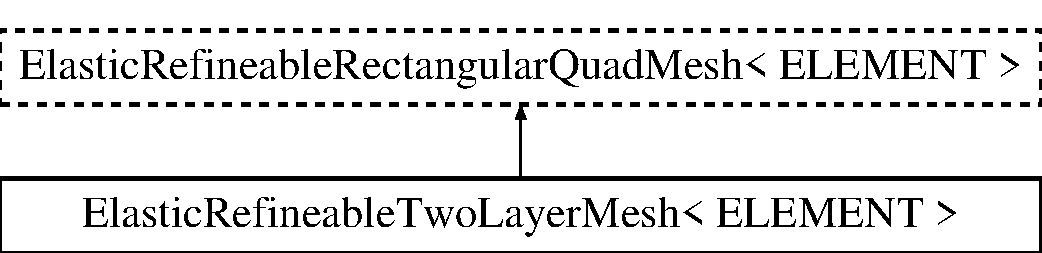
\includegraphics[height=2.000000cm]{classElasticRefineableTwoLayerMesh}
\end{center}
\end{figure}
\subsection*{Public Member Functions}
\begin{DoxyCompactItemize}
\item 
\hyperlink{classElasticRefineableTwoLayerMesh_a868e53937a6cd94e2ff252fe2002a216}{Elastic\+Refineable\+Two\+Layer\+Mesh} (const unsigned \&nx, const unsigned \&ny1, const unsigned \&ny2, const double \&lx, const double \&h1, const double \&h2, Time\+Stepper $\ast$time\+\_\+stepper\+\_\+pt=\&Mesh\+::\+Default\+\_\+\+Time\+Stepper)
\begin{DoxyCompactList}\small\item\em Constructor\+: Pass number of elements in x-\/direction, number of elements in y-\/direction in bottom and top layer, respectively, axial length and height of top and bottom layers, and pointer to timestepper (defaults to Steady timestepper) \end{DoxyCompactList}\end{DoxyCompactItemize}


\subsection{Detailed Description}
\subsubsection*{template$<$class E\+L\+E\+M\+E\+NT$>$\newline
class Elastic\+Refineable\+Two\+Layer\+Mesh$<$ E\+L\+E\+M\+E\+N\+T $>$}

Two layer mesh which employs a pseudo-\/solid node-\/update strategy. This class is essentially a wrapper to an Elastic\+Refineable\+Rectangular\+Quad\+Mesh, with an additional boundary to represent the interface between the two fluid layers. 

Definition at line 110 of file elastic\+\_\+two\+\_\+layer\+\_\+interface\+\_\+axisym.\+cc.



\subsection{Constructor \& Destructor Documentation}
\mbox{\Hypertarget{classElasticRefineableTwoLayerMesh_a868e53937a6cd94e2ff252fe2002a216}\label{classElasticRefineableTwoLayerMesh_a868e53937a6cd94e2ff252fe2002a216}} 
\index{Elastic\+Refineable\+Two\+Layer\+Mesh@{Elastic\+Refineable\+Two\+Layer\+Mesh}!Elastic\+Refineable\+Two\+Layer\+Mesh@{Elastic\+Refineable\+Two\+Layer\+Mesh}}
\index{Elastic\+Refineable\+Two\+Layer\+Mesh@{Elastic\+Refineable\+Two\+Layer\+Mesh}!Elastic\+Refineable\+Two\+Layer\+Mesh@{Elastic\+Refineable\+Two\+Layer\+Mesh}}
\subsubsection{\texorpdfstring{Elastic\+Refineable\+Two\+Layer\+Mesh()}{ElasticRefineableTwoLayerMesh()}}
{\footnotesize\ttfamily template$<$class E\+L\+E\+M\+E\+NT$>$ \\
\hyperlink{classElasticRefineableTwoLayerMesh}{Elastic\+Refineable\+Two\+Layer\+Mesh}$<$ E\+L\+E\+M\+E\+NT $>$\+::\hyperlink{classElasticRefineableTwoLayerMesh}{Elastic\+Refineable\+Two\+Layer\+Mesh} (\begin{DoxyParamCaption}\item[{const unsigned \&}]{nx,  }\item[{const unsigned \&}]{ny1,  }\item[{const unsigned \&}]{ny2,  }\item[{const double \&}]{lx,  }\item[{const double \&}]{h1,  }\item[{const double \&}]{h2,  }\item[{Time\+Stepper $\ast$}]{time\+\_\+stepper\+\_\+pt = {\ttfamily \&Mesh\+:\+:Default\+\_\+TimeStepper} }\end{DoxyParamCaption})\hspace{0.3cm}{\ttfamily [inline]}}



Constructor\+: Pass number of elements in x-\/direction, number of elements in y-\/direction in bottom and top layer, respectively, axial length and height of top and bottom layers, and pointer to timestepper (defaults to Steady timestepper) 



Definition at line 120 of file elastic\+\_\+two\+\_\+layer\+\_\+interface\+\_\+axisym.\+cc.



The documentation for this class was generated from the following file\+:\begin{DoxyCompactItemize}
\item 
\hyperlink{elastic__two__layer__interface__axisym_8cc}{elastic\+\_\+two\+\_\+layer\+\_\+interface\+\_\+axisym.\+cc}\end{DoxyCompactItemize}

\hypertarget{classInterfaceProblem}{}\section{Interface\+Problem$<$ E\+L\+E\+M\+E\+NT, T\+I\+M\+E\+S\+T\+E\+P\+P\+ER $>$ Class Template Reference}
\label{classInterfaceProblem}\index{Interface\+Problem$<$ E\+L\+E\+M\+E\+N\+T, T\+I\+M\+E\+S\+T\+E\+P\+P\+E\+R $>$@{Interface\+Problem$<$ E\+L\+E\+M\+E\+N\+T, T\+I\+M\+E\+S\+T\+E\+P\+P\+E\+R $>$}}
Inheritance diagram for Interface\+Problem$<$ E\+L\+E\+M\+E\+NT, T\+I\+M\+E\+S\+T\+E\+P\+P\+ER $>$\+:\begin{figure}[H]
\begin{center}
\leavevmode
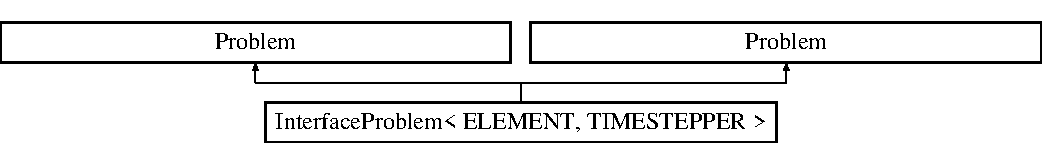
\includegraphics[height=1.924399cm]{classInterfaceProblem}
\end{center}
\end{figure}
\subsection*{Public Member Functions}
\begin{DoxyCompactItemize}
\item 
\hyperlink{classInterfaceProblem_a83023535d663a2a6558959f36bf6e1e7}{Interface\+Problem} (const unsigned \&n\+\_\+x, const unsigned \&n\+\_\+y, const double \&l\+\_\+x, const double \&h)
\begin{DoxyCompactList}\small\item\em Constructor for single fluid free surface problem. \end{DoxyCompactList}\item 
\hyperlink{classInterfaceProblem_a90c191f8046069099b199743e7ce7111}{$\sim$\+Interface\+Problem} ()
\begin{DoxyCompactList}\small\item\em Destructor (empty) \end{DoxyCompactList}\item 
void \hyperlink{classInterfaceProblem_a0d3af8378c4f0a6e38636be958c300d5}{set\+\_\+initial\+\_\+condition} ()
\begin{DoxyCompactList}\small\item\em Set initial conditions. \end{DoxyCompactList}\item 
void \hyperlink{classInterfaceProblem_a844445832ad7a32aa9f5d03ffdb40ebb}{set\+\_\+boundary\+\_\+conditions} ()
\begin{DoxyCompactList}\small\item\em Set boundary conditions. \end{DoxyCompactList}\item 
void \hyperlink{classInterfaceProblem_a49714e35e94f7d2af0b6ddd22b851f52}{doc\+\_\+solution} (Doc\+Info \&doc\+\_\+info)
\begin{DoxyCompactList}\small\item\em Document the solution. \end{DoxyCompactList}\item 
void \hyperlink{classInterfaceProblem_adf1f4e43d10939e4323e0e315b711085}{unsteady\+\_\+run} (const double \&t\+\_\+max, const double \&dt)
\begin{DoxyCompactList}\small\item\em Do unsteady run up to maximum time t\+\_\+max with given timestep dt. \end{DoxyCompactList}\item 
\hyperlink{classInterfaceProblem_a83023535d663a2a6558959f36bf6e1e7}{Interface\+Problem} (const unsigned \&n\+\_\+x, const unsigned \&n\+\_\+y, const double \&l\+\_\+x, const double \&h)
\item 
\hyperlink{classInterfaceProblem_a90c191f8046069099b199743e7ce7111}{$\sim$\+Interface\+Problem} ()
\begin{DoxyCompactList}\small\item\em Destructor (empty) \end{DoxyCompactList}\item 
void \hyperlink{classInterfaceProblem_a0d3af8378c4f0a6e38636be958c300d5}{set\+\_\+initial\+\_\+condition} ()
\begin{DoxyCompactList}\small\item\em Set initial conditions. \end{DoxyCompactList}\item 
void \hyperlink{classInterfaceProblem_a844445832ad7a32aa9f5d03ffdb40ebb}{set\+\_\+boundary\+\_\+conditions} ()
\begin{DoxyCompactList}\small\item\em Set boundary conditions. \end{DoxyCompactList}\item 
void \hyperlink{classInterfaceProblem_a49714e35e94f7d2af0b6ddd22b851f52}{doc\+\_\+solution} (Doc\+Info \&doc\+\_\+info)
\begin{DoxyCompactList}\small\item\em Doc the solution. \end{DoxyCompactList}\item 
void \hyperlink{classInterfaceProblem_adf1f4e43d10939e4323e0e315b711085}{unsteady\+\_\+run} (const double \&t\+\_\+max, const double \&dt)
\begin{DoxyCompactList}\small\item\em Do unsteady run up to maximum time t\+\_\+max with given timestep dt. \end{DoxyCompactList}\end{DoxyCompactItemize}
\subsection*{Public Attributes}
\begin{DoxyCompactItemize}
\item 
Single\+Layer\+Spine\+Mesh$<$ E\+L\+E\+M\+E\+NT $>$ $\ast$ \hyperlink{classInterfaceProblem_a3e9ad7667f6f978a1e7c4c55e8e69e6d}{Bulk\+\_\+mesh\+\_\+pt}
\begin{DoxyCompactList}\small\item\em The bulk fluid mesh, complete with spines and update information. \end{DoxyCompactList}\end{DoxyCompactItemize}
\subsection*{Private Member Functions}
\begin{DoxyCompactItemize}
\item 
void \hyperlink{classInterfaceProblem_ade63c8a74f666edf530460b989968b4f}{actions\+\_\+before\+\_\+newton\+\_\+solve} ()
\begin{DoxyCompactList}\small\item\em No actions required before solve step. \end{DoxyCompactList}\item 
void \hyperlink{classInterfaceProblem_aedc2e58b3d2f5f8c898a21ba2d245cee}{actions\+\_\+after\+\_\+newton\+\_\+solve} ()
\begin{DoxyCompactList}\small\item\em No actions required after solve step. \end{DoxyCompactList}\item 
void \hyperlink{classInterfaceProblem_ae3ec75fcc8ccca97207dc7eca23b1cce}{actions\+\_\+before\+\_\+implicit\+\_\+timestep} ()
\begin{DoxyCompactList}\small\item\em Actions before the timestep\+: For maximum stability, reset the current nodal positions to be the \char`\"{}stress-\/free\char`\"{} ones. \end{DoxyCompactList}\item 
void \hyperlink{classInterfaceProblem_a2319232b08d9df1ab473f6cbd40939d5}{deform\+\_\+free\+\_\+surface} (const double \&epsilon, const unsigned \&n\+\_\+periods)
\begin{DoxyCompactList}\small\item\em Deform the mesh/free surface to a prescribed function. \end{DoxyCompactList}\item 
void \hyperlink{classInterfaceProblem_ab4193771472aefce4cd67261491cc344}{actions\+\_\+before\+\_\+newton\+\_\+convergence\+\_\+check} ()
\begin{DoxyCompactList}\small\item\em Spine heights/lengths are unknowns in the problem so their values get corrected during each Newton step. However, changing their value does not automatically change the nodal positions, so we need to update all of them here. \end{DoxyCompactList}\item 
void \hyperlink{classInterfaceProblem_ade63c8a74f666edf530460b989968b4f}{actions\+\_\+before\+\_\+newton\+\_\+solve} ()
\begin{DoxyCompactList}\small\item\em No actions required before solve step. \end{DoxyCompactList}\item 
void \hyperlink{classInterfaceProblem_aedc2e58b3d2f5f8c898a21ba2d245cee}{actions\+\_\+after\+\_\+newton\+\_\+solve} ()
\begin{DoxyCompactList}\small\item\em Update after solve can remain empty, because the update is performed automatically after every Newton step. \end{DoxyCompactList}\item 
void \hyperlink{classInterfaceProblem_a2319232b08d9df1ab473f6cbd40939d5}{deform\+\_\+free\+\_\+surface} (const double \&epsilon, const unsigned \&n\+\_\+periods)
\begin{DoxyCompactList}\small\item\em Deform the mesh/free surface to a prescribed function. \end{DoxyCompactList}\end{DoxyCompactItemize}
\subsection*{Private Attributes}
\begin{DoxyCompactItemize}
\item 
Elastic\+Rectangular\+Quad\+Mesh$<$ E\+L\+E\+M\+E\+NT $>$ $\ast$ \hyperlink{classInterfaceProblem_af580057bd9cc1d05a67401c9e5e178c2}{Bulk\+\_\+mesh\+\_\+pt}
\begin{DoxyCompactList}\small\item\em Pointer to the (specific) \char`\"{}bulk\char`\"{} mesh. \end{DoxyCompactList}\item 
Mesh $\ast$ \hyperlink{classInterfaceProblem_a011c7b4f2307ff909f64dc158e8fc674}{Surface\+\_\+mesh\+\_\+pt}
\begin{DoxyCompactList}\small\item\em Pointer to the \char`\"{}surface\char`\"{} mesh. \end{DoxyCompactList}\item 
Constitutive\+Law $\ast$ \hyperlink{classInterfaceProblem_a5bf645cbdbf7775ab6438be324caf3c3}{Constitutive\+\_\+law\+\_\+pt}
\item 
double \hyperlink{classInterfaceProblem_a9b5070b479a79546b983bd7027917e93}{Lx}
\begin{DoxyCompactList}\small\item\em Width of domain. \end{DoxyCompactList}\item 
ofstream \hyperlink{classInterfaceProblem_a45e3bf3b44bcbeefab21a3598bef6179}{Trace\+\_\+file}
\begin{DoxyCompactList}\small\item\em Trace file. \end{DoxyCompactList}\end{DoxyCompactItemize}


\subsection{Detailed Description}
\subsubsection*{template$<$class E\+L\+E\+M\+E\+NT, class T\+I\+M\+E\+S\+T\+E\+P\+P\+ER$>$\newline
class Interface\+Problem$<$ E\+L\+E\+M\+E\+N\+T, T\+I\+M\+E\+S\+T\+E\+P\+P\+E\+R $>$}

Single fluid free surface problem in a rectangular domain which is periodic in the x direction 

Definition at line 96 of file elastic\+\_\+single\+\_\+layer.\+cc.



\subsection{Constructor \& Destructor Documentation}
\mbox{\Hypertarget{classInterfaceProblem_a83023535d663a2a6558959f36bf6e1e7}\label{classInterfaceProblem_a83023535d663a2a6558959f36bf6e1e7}} 
\index{Interface\+Problem@{Interface\+Problem}!Interface\+Problem@{Interface\+Problem}}
\index{Interface\+Problem@{Interface\+Problem}!Interface\+Problem@{Interface\+Problem}}
\subsubsection{\texorpdfstring{Interface\+Problem()}{InterfaceProblem()}\hspace{0.1cm}{\footnotesize\ttfamily [1/2]}}
{\footnotesize\ttfamily template$<$class E\+L\+E\+M\+E\+NT , class T\+I\+M\+E\+S\+T\+E\+P\+P\+ER $>$ \\
\hyperlink{classInterfaceProblem}{Interface\+Problem}$<$ E\+L\+E\+M\+E\+NT, T\+I\+M\+E\+S\+T\+E\+P\+P\+ER $>$\+::\hyperlink{classInterfaceProblem}{Interface\+Problem} (\begin{DoxyParamCaption}\item[{const unsigned \&}]{n\+\_\+x,  }\item[{const unsigned \&}]{n\+\_\+y,  }\item[{const double \&}]{l\+\_\+x,  }\item[{const double \&}]{h }\end{DoxyParamCaption})}



Constructor for single fluid free surface problem. 

Constructor\+: Pass the number of elements and the lengths of the domain in the x and y directions (h is the height of the fluid layer i.\+e. the length of the domain in the y direction) 

Definition at line 164 of file elastic\+\_\+single\+\_\+layer.\+cc.



References Interface\+Problem$<$ E\+L\+E\+M\+E\+N\+T, T\+I\+M\+E\+S\+T\+E\+P\+P\+E\+R $>$\+::\+Bulk\+\_\+mesh\+\_\+pt, Global\+\_\+\+Physical\+\_\+\+Variables\+::\+Ca, Interface\+Problem$<$ E\+L\+E\+M\+E\+N\+T, T\+I\+M\+E\+S\+T\+E\+P\+P\+E\+R $>$\+::\+Constitutive\+\_\+law\+\_\+pt, Global\+\_\+\+Physical\+\_\+\+Variables\+::\+G(), Global\+\_\+\+Physical\+\_\+\+Variables\+::\+Nu, Global\+\_\+\+Physical\+\_\+\+Variables\+::\+Re, Global\+\_\+\+Physical\+\_\+\+Variables\+::\+Re\+Inv\+Fr, Global\+\_\+\+Physical\+\_\+\+Variables\+::\+Re\+St, Interface\+Problem$<$ E\+L\+E\+M\+E\+N\+T, T\+I\+M\+E\+S\+T\+E\+P\+P\+E\+R $>$\+::set\+\_\+boundary\+\_\+conditions(), Global\+\_\+\+Physical\+\_\+\+Variables\+::\+St, and Interface\+Problem$<$ E\+L\+E\+M\+E\+N\+T, T\+I\+M\+E\+S\+T\+E\+P\+P\+E\+R $>$\+::\+Surface\+\_\+mesh\+\_\+pt.



Referenced by Interface\+Problem$<$ E\+L\+E\+M\+E\+N\+T, T\+I\+M\+E\+S\+T\+E\+P\+P\+E\+R $>$\+::actions\+\_\+after\+\_\+newton\+\_\+solve().

\mbox{\Hypertarget{classInterfaceProblem_a90c191f8046069099b199743e7ce7111}\label{classInterfaceProblem_a90c191f8046069099b199743e7ce7111}} 
\index{Interface\+Problem@{Interface\+Problem}!````~Interface\+Problem@{$\sim$\+Interface\+Problem}}
\index{````~Interface\+Problem@{$\sim$\+Interface\+Problem}!Interface\+Problem@{Interface\+Problem}}
\subsubsection{\texorpdfstring{$\sim$\+Interface\+Problem()}{~InterfaceProblem()}\hspace{0.1cm}{\footnotesize\ttfamily [1/2]}}
{\footnotesize\ttfamily template$<$class E\+L\+E\+M\+E\+NT, class T\+I\+M\+E\+S\+T\+E\+P\+P\+ER$>$ \\
\hyperlink{classInterfaceProblem}{Interface\+Problem}$<$ E\+L\+E\+M\+E\+NT, T\+I\+M\+E\+S\+T\+E\+P\+P\+ER $>$\+::$\sim$\hyperlink{classInterfaceProblem}{Interface\+Problem} (\begin{DoxyParamCaption}{ }\end{DoxyParamCaption})\hspace{0.3cm}{\ttfamily [inline]}}



Destructor (empty) 



Definition at line 108 of file elastic\+\_\+single\+\_\+layer.\+cc.

\mbox{\Hypertarget{classInterfaceProblem_a83023535d663a2a6558959f36bf6e1e7}\label{classInterfaceProblem_a83023535d663a2a6558959f36bf6e1e7}} 
\index{Interface\+Problem@{Interface\+Problem}!Interface\+Problem@{Interface\+Problem}}
\index{Interface\+Problem@{Interface\+Problem}!Interface\+Problem@{Interface\+Problem}}
\subsubsection{\texorpdfstring{Interface\+Problem()}{InterfaceProblem()}\hspace{0.1cm}{\footnotesize\ttfamily [2/2]}}
{\footnotesize\ttfamily template$<$class E\+L\+E\+M\+E\+NT, class T\+I\+M\+E\+S\+T\+E\+P\+P\+ER$>$ \\
\hyperlink{classInterfaceProblem}{Interface\+Problem}$<$ E\+L\+E\+M\+E\+NT, T\+I\+M\+E\+S\+T\+E\+P\+P\+ER $>$\+::\hyperlink{classInterfaceProblem}{Interface\+Problem} (\begin{DoxyParamCaption}\item[{const unsigned \&}]{n\+\_\+x,  }\item[{const unsigned \&}]{n\+\_\+y,  }\item[{const double \&}]{l\+\_\+x,  }\item[{const double \&}]{h }\end{DoxyParamCaption})}

Constructor\+: Pass the number of elements and the lengths of the domain in the x and y directions (h is the height of the fluid layer i.\+e. the length of the domain in the y direction) \mbox{\Hypertarget{classInterfaceProblem_a90c191f8046069099b199743e7ce7111}\label{classInterfaceProblem_a90c191f8046069099b199743e7ce7111}} 
\index{Interface\+Problem@{Interface\+Problem}!````~Interface\+Problem@{$\sim$\+Interface\+Problem}}
\index{````~Interface\+Problem@{$\sim$\+Interface\+Problem}!Interface\+Problem@{Interface\+Problem}}
\subsubsection{\texorpdfstring{$\sim$\+Interface\+Problem()}{~InterfaceProblem()}\hspace{0.1cm}{\footnotesize\ttfamily [2/2]}}
{\footnotesize\ttfamily template$<$class E\+L\+E\+M\+E\+NT, class T\+I\+M\+E\+S\+T\+E\+P\+P\+ER$>$ \\
\hyperlink{classInterfaceProblem}{Interface\+Problem}$<$ E\+L\+E\+M\+E\+NT, T\+I\+M\+E\+S\+T\+E\+P\+P\+ER $>$\+::$\sim$\hyperlink{classInterfaceProblem}{Interface\+Problem} (\begin{DoxyParamCaption}{ }\end{DoxyParamCaption})\hspace{0.3cm}{\ttfamily [inline]}}



Destructor (empty) 



Definition at line 99 of file spine\+\_\+single\+\_\+layer.\+cc.



\subsection{Member Function Documentation}
\mbox{\Hypertarget{classInterfaceProblem_aedc2e58b3d2f5f8c898a21ba2d245cee}\label{classInterfaceProblem_aedc2e58b3d2f5f8c898a21ba2d245cee}} 
\index{Interface\+Problem@{Interface\+Problem}!actions\+\_\+after\+\_\+newton\+\_\+solve@{actions\+\_\+after\+\_\+newton\+\_\+solve}}
\index{actions\+\_\+after\+\_\+newton\+\_\+solve@{actions\+\_\+after\+\_\+newton\+\_\+solve}!Interface\+Problem@{Interface\+Problem}}
\subsubsection{\texorpdfstring{actions\+\_\+after\+\_\+newton\+\_\+solve()}{actions\_after\_newton\_solve()}\hspace{0.1cm}{\footnotesize\ttfamily [1/2]}}
{\footnotesize\ttfamily template$<$class E\+L\+E\+M\+E\+NT, class T\+I\+M\+E\+S\+T\+E\+P\+P\+ER$>$ \\
void \hyperlink{classInterfaceProblem}{Interface\+Problem}$<$ E\+L\+E\+M\+E\+NT, T\+I\+M\+E\+S\+T\+E\+P\+P\+ER $>$\+::actions\+\_\+after\+\_\+newton\+\_\+solve (\begin{DoxyParamCaption}{ }\end{DoxyParamCaption})\hspace{0.3cm}{\ttfamily [inline]}, {\ttfamily [private]}}



No actions required after solve step. 



Definition at line 128 of file elastic\+\_\+single\+\_\+layer.\+cc.

\mbox{\Hypertarget{classInterfaceProblem_aedc2e58b3d2f5f8c898a21ba2d245cee}\label{classInterfaceProblem_aedc2e58b3d2f5f8c898a21ba2d245cee}} 
\index{Interface\+Problem@{Interface\+Problem}!actions\+\_\+after\+\_\+newton\+\_\+solve@{actions\+\_\+after\+\_\+newton\+\_\+solve}}
\index{actions\+\_\+after\+\_\+newton\+\_\+solve@{actions\+\_\+after\+\_\+newton\+\_\+solve}!Interface\+Problem@{Interface\+Problem}}
\subsubsection{\texorpdfstring{actions\+\_\+after\+\_\+newton\+\_\+solve()}{actions\_after\_newton\_solve()}\hspace{0.1cm}{\footnotesize\ttfamily [2/2]}}
{\footnotesize\ttfamily template$<$class E\+L\+E\+M\+E\+NT, class T\+I\+M\+E\+S\+T\+E\+P\+P\+ER$>$ \\
void \hyperlink{classInterfaceProblem}{Interface\+Problem}$<$ E\+L\+E\+M\+E\+NT, T\+I\+M\+E\+S\+T\+E\+P\+P\+ER $>$\+::actions\+\_\+after\+\_\+newton\+\_\+solve (\begin{DoxyParamCaption}{ }\end{DoxyParamCaption})\hspace{0.3cm}{\ttfamily [inline]}, {\ttfamily [private]}}



Update after solve can remain empty, because the update is performed automatically after every Newton step. 



Definition at line 135 of file spine\+\_\+single\+\_\+layer.\+cc.



References Global\+\_\+\+Physical\+\_\+\+Variables\+::\+Ca, Interface\+Problem$<$ E\+L\+E\+M\+E\+N\+T, T\+I\+M\+E\+S\+T\+E\+P\+P\+E\+R $>$\+::deform\+\_\+free\+\_\+surface(), Interface\+Problem$<$ E\+L\+E\+M\+E\+N\+T, T\+I\+M\+E\+S\+T\+E\+P\+P\+E\+R $>$\+::doc\+\_\+solution(), Global\+\_\+\+Physical\+\_\+\+Variables\+::\+G(), Interface\+Problem$<$ E\+L\+E\+M\+E\+N\+T, T\+I\+M\+E\+S\+T\+E\+P\+P\+E\+R $>$\+::\+Interface\+Problem(), Global\+\_\+\+Physical\+\_\+\+Variables\+::\+Re, Global\+\_\+\+Physical\+\_\+\+Variables\+::\+Re\+Inv\+Fr, Global\+\_\+\+Physical\+\_\+\+Variables\+::\+Re\+St, Interface\+Problem$<$ E\+L\+E\+M\+E\+N\+T, T\+I\+M\+E\+S\+T\+E\+P\+P\+E\+R $>$\+::set\+\_\+boundary\+\_\+conditions(), Interface\+Problem$<$ E\+L\+E\+M\+E\+N\+T, T\+I\+M\+E\+S\+T\+E\+P\+P\+E\+R $>$\+::set\+\_\+initial\+\_\+condition(), Global\+\_\+\+Physical\+\_\+\+Variables\+::\+St, and Interface\+Problem$<$ E\+L\+E\+M\+E\+N\+T, T\+I\+M\+E\+S\+T\+E\+P\+P\+E\+R $>$\+::unsteady\+\_\+run().

\mbox{\Hypertarget{classInterfaceProblem_ae3ec75fcc8ccca97207dc7eca23b1cce}\label{classInterfaceProblem_ae3ec75fcc8ccca97207dc7eca23b1cce}} 
\index{Interface\+Problem@{Interface\+Problem}!actions\+\_\+before\+\_\+implicit\+\_\+timestep@{actions\+\_\+before\+\_\+implicit\+\_\+timestep}}
\index{actions\+\_\+before\+\_\+implicit\+\_\+timestep@{actions\+\_\+before\+\_\+implicit\+\_\+timestep}!Interface\+Problem@{Interface\+Problem}}
\subsubsection{\texorpdfstring{actions\+\_\+before\+\_\+implicit\+\_\+timestep()}{actions\_before\_implicit\_timestep()}}
{\footnotesize\ttfamily template$<$class E\+L\+E\+M\+E\+NT, class T\+I\+M\+E\+S\+T\+E\+P\+P\+ER$>$ \\
void \hyperlink{classInterfaceProblem}{Interface\+Problem}$<$ E\+L\+E\+M\+E\+NT, T\+I\+M\+E\+S\+T\+E\+P\+P\+ER $>$\+::actions\+\_\+before\+\_\+implicit\+\_\+timestep (\begin{DoxyParamCaption}{ }\end{DoxyParamCaption})\hspace{0.3cm}{\ttfamily [inline]}, {\ttfamily [private]}}



Actions before the timestep\+: For maximum stability, reset the current nodal positions to be the \char`\"{}stress-\/free\char`\"{} ones. 



Definition at line 132 of file elastic\+\_\+single\+\_\+layer.\+cc.

\mbox{\Hypertarget{classInterfaceProblem_ab4193771472aefce4cd67261491cc344}\label{classInterfaceProblem_ab4193771472aefce4cd67261491cc344}} 
\index{Interface\+Problem@{Interface\+Problem}!actions\+\_\+before\+\_\+newton\+\_\+convergence\+\_\+check@{actions\+\_\+before\+\_\+newton\+\_\+convergence\+\_\+check}}
\index{actions\+\_\+before\+\_\+newton\+\_\+convergence\+\_\+check@{actions\+\_\+before\+\_\+newton\+\_\+convergence\+\_\+check}!Interface\+Problem@{Interface\+Problem}}
\subsubsection{\texorpdfstring{actions\+\_\+before\+\_\+newton\+\_\+convergence\+\_\+check()}{actions\_before\_newton\_convergence\_check()}}
{\footnotesize\ttfamily template$<$class E\+L\+E\+M\+E\+NT, class T\+I\+M\+E\+S\+T\+E\+P\+P\+ER$>$ \\
void \hyperlink{classInterfaceProblem}{Interface\+Problem}$<$ E\+L\+E\+M\+E\+NT, T\+I\+M\+E\+S\+T\+E\+P\+P\+ER $>$\+::actions\+\_\+before\+\_\+newton\+\_\+convergence\+\_\+check (\begin{DoxyParamCaption}{ }\end{DoxyParamCaption})\hspace{0.3cm}{\ttfamily [inline]}, {\ttfamily [private]}}



Spine heights/lengths are unknowns in the problem so their values get corrected during each Newton step. However, changing their value does not automatically change the nodal positions, so we need to update all of them here. 



Definition at line 125 of file spine\+\_\+single\+\_\+layer.\+cc.

\mbox{\Hypertarget{classInterfaceProblem_ade63c8a74f666edf530460b989968b4f}\label{classInterfaceProblem_ade63c8a74f666edf530460b989968b4f}} 
\index{Interface\+Problem@{Interface\+Problem}!actions\+\_\+before\+\_\+newton\+\_\+solve@{actions\+\_\+before\+\_\+newton\+\_\+solve}}
\index{actions\+\_\+before\+\_\+newton\+\_\+solve@{actions\+\_\+before\+\_\+newton\+\_\+solve}!Interface\+Problem@{Interface\+Problem}}
\subsubsection{\texorpdfstring{actions\+\_\+before\+\_\+newton\+\_\+solve()}{actions\_before\_newton\_solve()}\hspace{0.1cm}{\footnotesize\ttfamily [1/2]}}
{\footnotesize\ttfamily template$<$class E\+L\+E\+M\+E\+NT, class T\+I\+M\+E\+S\+T\+E\+P\+P\+ER$>$ \\
void \hyperlink{classInterfaceProblem}{Interface\+Problem}$<$ E\+L\+E\+M\+E\+NT, T\+I\+M\+E\+S\+T\+E\+P\+P\+ER $>$\+::actions\+\_\+before\+\_\+newton\+\_\+solve (\begin{DoxyParamCaption}{ }\end{DoxyParamCaption})\hspace{0.3cm}{\ttfamily [inline]}, {\ttfamily [private]}}



No actions required before solve step. 



Definition at line 125 of file elastic\+\_\+single\+\_\+layer.\+cc.

\mbox{\Hypertarget{classInterfaceProblem_ade63c8a74f666edf530460b989968b4f}\label{classInterfaceProblem_ade63c8a74f666edf530460b989968b4f}} 
\index{Interface\+Problem@{Interface\+Problem}!actions\+\_\+before\+\_\+newton\+\_\+solve@{actions\+\_\+before\+\_\+newton\+\_\+solve}}
\index{actions\+\_\+before\+\_\+newton\+\_\+solve@{actions\+\_\+before\+\_\+newton\+\_\+solve}!Interface\+Problem@{Interface\+Problem}}
\subsubsection{\texorpdfstring{actions\+\_\+before\+\_\+newton\+\_\+solve()}{actions\_before\_newton\_solve()}\hspace{0.1cm}{\footnotesize\ttfamily [2/2]}}
{\footnotesize\ttfamily template$<$class E\+L\+E\+M\+E\+NT, class T\+I\+M\+E\+S\+T\+E\+P\+P\+ER$>$ \\
void \hyperlink{classInterfaceProblem}{Interface\+Problem}$<$ E\+L\+E\+M\+E\+NT, T\+I\+M\+E\+S\+T\+E\+P\+P\+ER $>$\+::actions\+\_\+before\+\_\+newton\+\_\+solve (\begin{DoxyParamCaption}{ }\end{DoxyParamCaption})\hspace{0.3cm}{\ttfamily [inline]}, {\ttfamily [private]}}



No actions required before solve step. 



Definition at line 131 of file spine\+\_\+single\+\_\+layer.\+cc.

\mbox{\Hypertarget{classInterfaceProblem_a2319232b08d9df1ab473f6cbd40939d5}\label{classInterfaceProblem_a2319232b08d9df1ab473f6cbd40939d5}} 
\index{Interface\+Problem@{Interface\+Problem}!deform\+\_\+free\+\_\+surface@{deform\+\_\+free\+\_\+surface}}
\index{deform\+\_\+free\+\_\+surface@{deform\+\_\+free\+\_\+surface}!Interface\+Problem@{Interface\+Problem}}
\subsubsection{\texorpdfstring{deform\+\_\+free\+\_\+surface()}{deform\_free\_surface()}\hspace{0.1cm}{\footnotesize\ttfamily [1/2]}}
{\footnotesize\ttfamily template$<$class E\+L\+E\+M\+E\+NT , class T\+I\+M\+E\+S\+T\+E\+P\+P\+ER $>$ \\
void \hyperlink{classInterfaceProblem}{Interface\+Problem}$<$ E\+L\+E\+M\+E\+NT, T\+I\+M\+E\+S\+T\+E\+P\+P\+ER $>$\+::deform\+\_\+free\+\_\+surface (\begin{DoxyParamCaption}\item[{const double \&}]{epsilon,  }\item[{const unsigned \&}]{n\+\_\+periods }\end{DoxyParamCaption})\hspace{0.3cm}{\ttfamily [private]}}



Deform the mesh/free surface to a prescribed function. 



Definition at line 408 of file elastic\+\_\+single\+\_\+layer.\+cc.



References Interface\+Problem$<$ E\+L\+E\+M\+E\+N\+T, T\+I\+M\+E\+S\+T\+E\+P\+P\+E\+R $>$\+::\+Bulk\+\_\+mesh\+\_\+pt, and Interface\+Problem$<$ E\+L\+E\+M\+E\+N\+T, T\+I\+M\+E\+S\+T\+E\+P\+P\+E\+R $>$\+::\+Lx.



Referenced by Interface\+Problem$<$ E\+L\+E\+M\+E\+N\+T, T\+I\+M\+E\+S\+T\+E\+P\+P\+E\+R $>$\+::actions\+\_\+after\+\_\+newton\+\_\+solve(), Interface\+Problem$<$ E\+L\+E\+M\+E\+N\+T, T\+I\+M\+E\+S\+T\+E\+P\+P\+E\+R $>$\+::set\+\_\+boundary\+\_\+conditions(), and Interface\+Problem$<$ E\+L\+E\+M\+E\+N\+T, T\+I\+M\+E\+S\+T\+E\+P\+P\+E\+R $>$\+::unsteady\+\_\+run().

\mbox{\Hypertarget{classInterfaceProblem_a2319232b08d9df1ab473f6cbd40939d5}\label{classInterfaceProblem_a2319232b08d9df1ab473f6cbd40939d5}} 
\index{Interface\+Problem@{Interface\+Problem}!deform\+\_\+free\+\_\+surface@{deform\+\_\+free\+\_\+surface}}
\index{deform\+\_\+free\+\_\+surface@{deform\+\_\+free\+\_\+surface}!Interface\+Problem@{Interface\+Problem}}
\subsubsection{\texorpdfstring{deform\+\_\+free\+\_\+surface()}{deform\_free\_surface()}\hspace{0.1cm}{\footnotesize\ttfamily [2/2]}}
{\footnotesize\ttfamily template$<$class E\+L\+E\+M\+E\+NT, class T\+I\+M\+E\+S\+T\+E\+P\+P\+ER$>$ \\
void \hyperlink{classInterfaceProblem}{Interface\+Problem}$<$ E\+L\+E\+M\+E\+NT, T\+I\+M\+E\+S\+T\+E\+P\+P\+ER $>$\+::deform\+\_\+free\+\_\+surface (\begin{DoxyParamCaption}\item[{const double \&}]{epsilon,  }\item[{const unsigned \&}]{n\+\_\+periods }\end{DoxyParamCaption})\hspace{0.3cm}{\ttfamily [private]}}



Deform the mesh/free surface to a prescribed function. 

\mbox{\Hypertarget{classInterfaceProblem_a49714e35e94f7d2af0b6ddd22b851f52}\label{classInterfaceProblem_a49714e35e94f7d2af0b6ddd22b851f52}} 
\index{Interface\+Problem@{Interface\+Problem}!doc\+\_\+solution@{doc\+\_\+solution}}
\index{doc\+\_\+solution@{doc\+\_\+solution}!Interface\+Problem@{Interface\+Problem}}
\subsubsection{\texorpdfstring{doc\+\_\+solution()}{doc\_solution()}\hspace{0.1cm}{\footnotesize\ttfamily [1/2]}}
{\footnotesize\ttfamily template$<$class E\+L\+E\+M\+E\+NT, class T\+I\+M\+E\+S\+T\+E\+P\+P\+ER$>$ \\
void \hyperlink{classInterfaceProblem}{Interface\+Problem}$<$ E\+L\+E\+M\+E\+NT, T\+I\+M\+E\+S\+T\+E\+P\+P\+ER $>$\+::doc\+\_\+solution (\begin{DoxyParamCaption}\item[{Doc\+Info \&}]{doc\+\_\+info }\end{DoxyParamCaption})}



Doc the solution. 

\mbox{\Hypertarget{classInterfaceProblem_a49714e35e94f7d2af0b6ddd22b851f52}\label{classInterfaceProblem_a49714e35e94f7d2af0b6ddd22b851f52}} 
\index{Interface\+Problem@{Interface\+Problem}!doc\+\_\+solution@{doc\+\_\+solution}}
\index{doc\+\_\+solution@{doc\+\_\+solution}!Interface\+Problem@{Interface\+Problem}}
\subsubsection{\texorpdfstring{doc\+\_\+solution()}{doc\_solution()}\hspace{0.1cm}{\footnotesize\ttfamily [2/2]}}
{\footnotesize\ttfamily template$<$class E\+L\+E\+M\+E\+NT , class T\+I\+M\+E\+S\+T\+E\+P\+P\+ER $>$ \\
void \hyperlink{classInterfaceProblem}{Interface\+Problem}$<$ E\+L\+E\+M\+E\+NT, T\+I\+M\+E\+S\+T\+E\+P\+P\+ER $>$\+::doc\+\_\+solution (\begin{DoxyParamCaption}\item[{Doc\+Info \&}]{doc\+\_\+info }\end{DoxyParamCaption})}



Document the solution. 

Doc the solution. 

Definition at line 436 of file elastic\+\_\+single\+\_\+layer.\+cc.



References Interface\+Problem$<$ E\+L\+E\+M\+E\+N\+T, T\+I\+M\+E\+S\+T\+E\+P\+P\+E\+R $>$\+::\+Bulk\+\_\+mesh\+\_\+pt, Interface\+Problem$<$ E\+L\+E\+M\+E\+N\+T, T\+I\+M\+E\+S\+T\+E\+P\+P\+E\+R $>$\+::\+Surface\+\_\+mesh\+\_\+pt, Interface\+Problem$<$ E\+L\+E\+M\+E\+N\+T, T\+I\+M\+E\+S\+T\+E\+P\+P\+E\+R $>$\+::\+Trace\+\_\+file, and Interface\+Problem$<$ E\+L\+E\+M\+E\+N\+T, T\+I\+M\+E\+S\+T\+E\+P\+P\+E\+R $>$\+::unsteady\+\_\+run().



Referenced by Interface\+Problem$<$ E\+L\+E\+M\+E\+N\+T, T\+I\+M\+E\+S\+T\+E\+P\+P\+E\+R $>$\+::actions\+\_\+after\+\_\+newton\+\_\+solve(), and Interface\+Problem$<$ E\+L\+E\+M\+E\+N\+T, T\+I\+M\+E\+S\+T\+E\+P\+P\+E\+R $>$\+::unsteady\+\_\+run().

\mbox{\Hypertarget{classInterfaceProblem_a844445832ad7a32aa9f5d03ffdb40ebb}\label{classInterfaceProblem_a844445832ad7a32aa9f5d03ffdb40ebb}} 
\index{Interface\+Problem@{Interface\+Problem}!set\+\_\+boundary\+\_\+conditions@{set\+\_\+boundary\+\_\+conditions}}
\index{set\+\_\+boundary\+\_\+conditions@{set\+\_\+boundary\+\_\+conditions}!Interface\+Problem@{Interface\+Problem}}
\subsubsection{\texorpdfstring{set\+\_\+boundary\+\_\+conditions()}{set\_boundary\_conditions()}\hspace{0.1cm}{\footnotesize\ttfamily [1/2]}}
{\footnotesize\ttfamily template$<$class E\+L\+E\+M\+E\+NT, class T\+I\+M\+E\+S\+T\+E\+P\+P\+ER$>$ \\
void \hyperlink{classInterfaceProblem}{Interface\+Problem}$<$ E\+L\+E\+M\+E\+NT, T\+I\+M\+E\+S\+T\+E\+P\+P\+ER $>$\+::set\+\_\+boundary\+\_\+conditions (\begin{DoxyParamCaption}{ }\end{DoxyParamCaption})}



Set boundary conditions. 

\mbox{\Hypertarget{classInterfaceProblem_a844445832ad7a32aa9f5d03ffdb40ebb}\label{classInterfaceProblem_a844445832ad7a32aa9f5d03ffdb40ebb}} 
\index{Interface\+Problem@{Interface\+Problem}!set\+\_\+boundary\+\_\+conditions@{set\+\_\+boundary\+\_\+conditions}}
\index{set\+\_\+boundary\+\_\+conditions@{set\+\_\+boundary\+\_\+conditions}!Interface\+Problem@{Interface\+Problem}}
\subsubsection{\texorpdfstring{set\+\_\+boundary\+\_\+conditions()}{set\_boundary\_conditions()}\hspace{0.1cm}{\footnotesize\ttfamily [2/2]}}
{\footnotesize\ttfamily template$<$class E\+L\+E\+M\+E\+NT , class T\+I\+M\+E\+S\+T\+E\+P\+P\+ER $>$ \\
void \hyperlink{classInterfaceProblem}{Interface\+Problem}$<$ E\+L\+E\+M\+E\+NT, T\+I\+M\+E\+S\+T\+E\+P\+P\+ER $>$\+::set\+\_\+boundary\+\_\+conditions (\begin{DoxyParamCaption}{ }\end{DoxyParamCaption})}



Set boundary conditions. 

Set boundary conditions\+: Set both velocity components to zero on the bottom (solid) wall and the horizontal component only to zero on the side (periodic) boundaries. 

Definition at line 370 of file elastic\+\_\+single\+\_\+layer.\+cc.



References Interface\+Problem$<$ E\+L\+E\+M\+E\+N\+T, T\+I\+M\+E\+S\+T\+E\+P\+P\+E\+R $>$\+::\+Bulk\+\_\+mesh\+\_\+pt, and Interface\+Problem$<$ E\+L\+E\+M\+E\+N\+T, T\+I\+M\+E\+S\+T\+E\+P\+P\+E\+R $>$\+::deform\+\_\+free\+\_\+surface().



Referenced by Interface\+Problem$<$ E\+L\+E\+M\+E\+N\+T, T\+I\+M\+E\+S\+T\+E\+P\+P\+E\+R $>$\+::actions\+\_\+after\+\_\+newton\+\_\+solve(), and Interface\+Problem$<$ E\+L\+E\+M\+E\+N\+T, T\+I\+M\+E\+S\+T\+E\+P\+P\+E\+R $>$\+::\+Interface\+Problem().

\mbox{\Hypertarget{classInterfaceProblem_a0d3af8378c4f0a6e38636be958c300d5}\label{classInterfaceProblem_a0d3af8378c4f0a6e38636be958c300d5}} 
\index{Interface\+Problem@{Interface\+Problem}!set\+\_\+initial\+\_\+condition@{set\+\_\+initial\+\_\+condition}}
\index{set\+\_\+initial\+\_\+condition@{set\+\_\+initial\+\_\+condition}!Interface\+Problem@{Interface\+Problem}}
\subsubsection{\texorpdfstring{set\+\_\+initial\+\_\+condition()}{set\_initial\_condition()}\hspace{0.1cm}{\footnotesize\ttfamily [1/2]}}
{\footnotesize\ttfamily template$<$class E\+L\+E\+M\+E\+NT, class T\+I\+M\+E\+S\+T\+E\+P\+P\+ER$>$ \\
void \hyperlink{classInterfaceProblem}{Interface\+Problem}$<$ E\+L\+E\+M\+E\+NT, T\+I\+M\+E\+S\+T\+E\+P\+P\+ER $>$\+::set\+\_\+initial\+\_\+condition (\begin{DoxyParamCaption}{ }\end{DoxyParamCaption})}



Set initial conditions. 

\mbox{\Hypertarget{classInterfaceProblem_a0d3af8378c4f0a6e38636be958c300d5}\label{classInterfaceProblem_a0d3af8378c4f0a6e38636be958c300d5}} 
\index{Interface\+Problem@{Interface\+Problem}!set\+\_\+initial\+\_\+condition@{set\+\_\+initial\+\_\+condition}}
\index{set\+\_\+initial\+\_\+condition@{set\+\_\+initial\+\_\+condition}!Interface\+Problem@{Interface\+Problem}}
\subsubsection{\texorpdfstring{set\+\_\+initial\+\_\+condition()}{set\_initial\_condition()}\hspace{0.1cm}{\footnotesize\ttfamily [2/2]}}
{\footnotesize\ttfamily template$<$class E\+L\+E\+M\+E\+NT , class T\+I\+M\+E\+S\+T\+E\+P\+P\+ER $>$ \\
void \hyperlink{classInterfaceProblem}{Interface\+Problem}$<$ E\+L\+E\+M\+E\+NT, T\+I\+M\+E\+S\+T\+E\+P\+P\+ER $>$\+::set\+\_\+initial\+\_\+condition (\begin{DoxyParamCaption}{ }\end{DoxyParamCaption})}



Set initial conditions. 

Set initial conditions\+: Set all nodal velocities to zero and initialise the previous velocities and nodal positions to correspond to an impulsive start. 

Definition at line 340 of file elastic\+\_\+single\+\_\+layer.\+cc.



Referenced by Interface\+Problem$<$ E\+L\+E\+M\+E\+N\+T, T\+I\+M\+E\+S\+T\+E\+P\+P\+E\+R $>$\+::actions\+\_\+after\+\_\+newton\+\_\+solve(), and Interface\+Problem$<$ E\+L\+E\+M\+E\+N\+T, T\+I\+M\+E\+S\+T\+E\+P\+P\+E\+R $>$\+::unsteady\+\_\+run().

\mbox{\Hypertarget{classInterfaceProblem_adf1f4e43d10939e4323e0e315b711085}\label{classInterfaceProblem_adf1f4e43d10939e4323e0e315b711085}} 
\index{Interface\+Problem@{Interface\+Problem}!unsteady\+\_\+run@{unsteady\+\_\+run}}
\index{unsteady\+\_\+run@{unsteady\+\_\+run}!Interface\+Problem@{Interface\+Problem}}
\subsubsection{\texorpdfstring{unsteady\+\_\+run()}{unsteady\_run()}\hspace{0.1cm}{\footnotesize\ttfamily [1/2]}}
{\footnotesize\ttfamily template$<$class E\+L\+E\+M\+E\+NT, class T\+I\+M\+E\+S\+T\+E\+P\+P\+ER$>$ \\
void \hyperlink{classInterfaceProblem}{Interface\+Problem}$<$ E\+L\+E\+M\+E\+NT, T\+I\+M\+E\+S\+T\+E\+P\+P\+ER $>$\+::unsteady\+\_\+run (\begin{DoxyParamCaption}\item[{const double \&}]{t\+\_\+max,  }\item[{const double \&}]{dt }\end{DoxyParamCaption})}



Do unsteady run up to maximum time t\+\_\+max with given timestep dt. 

\mbox{\Hypertarget{classInterfaceProblem_adf1f4e43d10939e4323e0e315b711085}\label{classInterfaceProblem_adf1f4e43d10939e4323e0e315b711085}} 
\index{Interface\+Problem@{Interface\+Problem}!unsteady\+\_\+run@{unsteady\+\_\+run}}
\index{unsteady\+\_\+run@{unsteady\+\_\+run}!Interface\+Problem@{Interface\+Problem}}
\subsubsection{\texorpdfstring{unsteady\+\_\+run()}{unsteady\_run()}\hspace{0.1cm}{\footnotesize\ttfamily [2/2]}}
{\footnotesize\ttfamily template$<$class E\+L\+E\+M\+E\+NT , class T\+I\+M\+E\+S\+T\+E\+P\+P\+ER $>$ \\
void \hyperlink{classInterfaceProblem}{Interface\+Problem}$<$ E\+L\+E\+M\+E\+NT, T\+I\+M\+E\+S\+T\+E\+P\+P\+ER $>$\+::unsteady\+\_\+run (\begin{DoxyParamCaption}\item[{const double \&}]{t\+\_\+max,  }\item[{const double \&}]{dt }\end{DoxyParamCaption})}



Do unsteady run up to maximum time t\+\_\+max with given timestep dt. 

Perform run up to specified time t\+\_\+max with given timestep dt. 

Definition at line 489 of file elastic\+\_\+single\+\_\+layer.\+cc.



References Interface\+Problem$<$ E\+L\+E\+M\+E\+N\+T, T\+I\+M\+E\+S\+T\+E\+P\+P\+E\+R $>$\+::deform\+\_\+free\+\_\+surface(), Interface\+Problem$<$ E\+L\+E\+M\+E\+N\+T, T\+I\+M\+E\+S\+T\+E\+P\+P\+E\+R $>$\+::doc\+\_\+solution(), Interface\+Problem$<$ E\+L\+E\+M\+E\+N\+T, T\+I\+M\+E\+S\+T\+E\+P\+P\+E\+R $>$\+::set\+\_\+initial\+\_\+condition(), and Interface\+Problem$<$ E\+L\+E\+M\+E\+N\+T, T\+I\+M\+E\+S\+T\+E\+P\+P\+E\+R $>$\+::\+Trace\+\_\+file.



Referenced by Interface\+Problem$<$ E\+L\+E\+M\+E\+N\+T, T\+I\+M\+E\+S\+T\+E\+P\+P\+E\+R $>$\+::actions\+\_\+after\+\_\+newton\+\_\+solve(), Interface\+Problem$<$ E\+L\+E\+M\+E\+N\+T, T\+I\+M\+E\+S\+T\+E\+P\+P\+E\+R $>$\+::doc\+\_\+solution(), and main().



\subsection{Member Data Documentation}
\mbox{\Hypertarget{classInterfaceProblem_a3e9ad7667f6f978a1e7c4c55e8e69e6d}\label{classInterfaceProblem_a3e9ad7667f6f978a1e7c4c55e8e69e6d}} 
\index{Interface\+Problem@{Interface\+Problem}!Bulk\+\_\+mesh\+\_\+pt@{Bulk\+\_\+mesh\+\_\+pt}}
\index{Bulk\+\_\+mesh\+\_\+pt@{Bulk\+\_\+mesh\+\_\+pt}!Interface\+Problem@{Interface\+Problem}}
\subsubsection{\texorpdfstring{Bulk\+\_\+mesh\+\_\+pt}{Bulk\_mesh\_pt}\hspace{0.1cm}{\footnotesize\ttfamily [1/2]}}
{\footnotesize\ttfamily template$<$class E\+L\+E\+M\+E\+NT, class T\+I\+M\+E\+S\+T\+E\+P\+P\+ER$>$ \\
Single\+Layer\+Spine\+Mesh$<$E\+L\+E\+M\+E\+NT$>$$\ast$ \hyperlink{classInterfaceProblem}{Interface\+Problem}$<$ E\+L\+E\+M\+E\+NT, T\+I\+M\+E\+S\+T\+E\+P\+P\+ER $>$\+::Bulk\+\_\+mesh\+\_\+pt}



The bulk fluid mesh, complete with spines and update information. 



Definition at line 114 of file spine\+\_\+single\+\_\+layer.\+cc.

\mbox{\Hypertarget{classInterfaceProblem_af580057bd9cc1d05a67401c9e5e178c2}\label{classInterfaceProblem_af580057bd9cc1d05a67401c9e5e178c2}} 
\index{Interface\+Problem@{Interface\+Problem}!Bulk\+\_\+mesh\+\_\+pt@{Bulk\+\_\+mesh\+\_\+pt}}
\index{Bulk\+\_\+mesh\+\_\+pt@{Bulk\+\_\+mesh\+\_\+pt}!Interface\+Problem@{Interface\+Problem}}
\subsubsection{\texorpdfstring{Bulk\+\_\+mesh\+\_\+pt}{Bulk\_mesh\_pt}\hspace{0.1cm}{\footnotesize\ttfamily [2/2]}}
{\footnotesize\ttfamily template$<$class E\+L\+E\+M\+E\+NT, class T\+I\+M\+E\+S\+T\+E\+P\+P\+ER$>$ \\
Elastic\+Rectangular\+Quad\+Mesh$<$E\+L\+E\+M\+E\+NT$>$$\ast$ \hyperlink{classInterfaceProblem}{Interface\+Problem}$<$ E\+L\+E\+M\+E\+NT, T\+I\+M\+E\+S\+T\+E\+P\+P\+ER $>$\+::Bulk\+\_\+mesh\+\_\+pt\hspace{0.3cm}{\ttfamily [private]}}



Pointer to the (specific) \char`\"{}bulk\char`\"{} mesh. 



Definition at line 141 of file elastic\+\_\+single\+\_\+layer.\+cc.



Referenced by Interface\+Problem$<$ E\+L\+E\+M\+E\+N\+T, T\+I\+M\+E\+S\+T\+E\+P\+P\+E\+R $>$\+::deform\+\_\+free\+\_\+surface(), Interface\+Problem$<$ E\+L\+E\+M\+E\+N\+T, T\+I\+M\+E\+S\+T\+E\+P\+P\+E\+R $>$\+::doc\+\_\+solution(), Interface\+Problem$<$ E\+L\+E\+M\+E\+N\+T, T\+I\+M\+E\+S\+T\+E\+P\+P\+E\+R $>$\+::\+Interface\+Problem(), and Interface\+Problem$<$ E\+L\+E\+M\+E\+N\+T, T\+I\+M\+E\+S\+T\+E\+P\+P\+E\+R $>$\+::set\+\_\+boundary\+\_\+conditions().

\mbox{\Hypertarget{classInterfaceProblem_a5bf645cbdbf7775ab6438be324caf3c3}\label{classInterfaceProblem_a5bf645cbdbf7775ab6438be324caf3c3}} 
\index{Interface\+Problem@{Interface\+Problem}!Constitutive\+\_\+law\+\_\+pt@{Constitutive\+\_\+law\+\_\+pt}}
\index{Constitutive\+\_\+law\+\_\+pt@{Constitutive\+\_\+law\+\_\+pt}!Interface\+Problem@{Interface\+Problem}}
\subsubsection{\texorpdfstring{Constitutive\+\_\+law\+\_\+pt}{Constitutive\_law\_pt}}
{\footnotesize\ttfamily template$<$class E\+L\+E\+M\+E\+NT, class T\+I\+M\+E\+S\+T\+E\+P\+P\+ER$>$ \\
Constitutive\+Law$\ast$ \hyperlink{classInterfaceProblem}{Interface\+Problem}$<$ E\+L\+E\+M\+E\+NT, T\+I\+M\+E\+S\+T\+E\+P\+P\+ER $>$\+::Constitutive\+\_\+law\+\_\+pt\hspace{0.3cm}{\ttfamily [private]}}



Definition at line 147 of file elastic\+\_\+single\+\_\+layer.\+cc.



Referenced by Interface\+Problem$<$ E\+L\+E\+M\+E\+N\+T, T\+I\+M\+E\+S\+T\+E\+P\+P\+E\+R $>$\+::\+Interface\+Problem().

\mbox{\Hypertarget{classInterfaceProblem_a9b5070b479a79546b983bd7027917e93}\label{classInterfaceProblem_a9b5070b479a79546b983bd7027917e93}} 
\index{Interface\+Problem@{Interface\+Problem}!Lx@{Lx}}
\index{Lx@{Lx}!Interface\+Problem@{Interface\+Problem}}
\subsubsection{\texorpdfstring{Lx}{Lx}}
{\footnotesize\ttfamily template$<$class E\+L\+E\+M\+E\+NT, class T\+I\+M\+E\+S\+T\+E\+P\+P\+ER$>$ \\
double \hyperlink{classInterfaceProblem}{Interface\+Problem}$<$ E\+L\+E\+M\+E\+NT, T\+I\+M\+E\+S\+T\+E\+P\+P\+ER $>$\+::Lx\hspace{0.3cm}{\ttfamily [private]}}



Width of domain. 



Definition at line 150 of file elastic\+\_\+single\+\_\+layer.\+cc.



Referenced by Interface\+Problem$<$ E\+L\+E\+M\+E\+N\+T, T\+I\+M\+E\+S\+T\+E\+P\+P\+E\+R $>$\+::deform\+\_\+free\+\_\+surface().

\mbox{\Hypertarget{classInterfaceProblem_a011c7b4f2307ff909f64dc158e8fc674}\label{classInterfaceProblem_a011c7b4f2307ff909f64dc158e8fc674}} 
\index{Interface\+Problem@{Interface\+Problem}!Surface\+\_\+mesh\+\_\+pt@{Surface\+\_\+mesh\+\_\+pt}}
\index{Surface\+\_\+mesh\+\_\+pt@{Surface\+\_\+mesh\+\_\+pt}!Interface\+Problem@{Interface\+Problem}}
\subsubsection{\texorpdfstring{Surface\+\_\+mesh\+\_\+pt}{Surface\_mesh\_pt}}
{\footnotesize\ttfamily template$<$class E\+L\+E\+M\+E\+NT, class T\+I\+M\+E\+S\+T\+E\+P\+P\+ER$>$ \\
Mesh $\ast$ \hyperlink{classInterfaceProblem}{Interface\+Problem}$<$ E\+L\+E\+M\+E\+NT, T\+I\+M\+E\+S\+T\+E\+P\+P\+ER $>$\+::Surface\+\_\+mesh\+\_\+pt\hspace{0.3cm}{\ttfamily [private]}}



Pointer to the \char`\"{}surface\char`\"{} mesh. 

The mesh that contains the free surface elements. 

Definition at line 144 of file elastic\+\_\+single\+\_\+layer.\+cc.



Referenced by Interface\+Problem$<$ E\+L\+E\+M\+E\+N\+T, T\+I\+M\+E\+S\+T\+E\+P\+P\+E\+R $>$\+::doc\+\_\+solution(), and Interface\+Problem$<$ E\+L\+E\+M\+E\+N\+T, T\+I\+M\+E\+S\+T\+E\+P\+P\+E\+R $>$\+::\+Interface\+Problem().

\mbox{\Hypertarget{classInterfaceProblem_a45e3bf3b44bcbeefab21a3598bef6179}\label{classInterfaceProblem_a45e3bf3b44bcbeefab21a3598bef6179}} 
\index{Interface\+Problem@{Interface\+Problem}!Trace\+\_\+file@{Trace\+\_\+file}}
\index{Trace\+\_\+file@{Trace\+\_\+file}!Interface\+Problem@{Interface\+Problem}}
\subsubsection{\texorpdfstring{Trace\+\_\+file}{Trace\_file}}
{\footnotesize\ttfamily template$<$class E\+L\+E\+M\+E\+NT, class T\+I\+M\+E\+S\+T\+E\+P\+P\+ER$>$ \\
ofstream \hyperlink{classInterfaceProblem}{Interface\+Problem}$<$ E\+L\+E\+M\+E\+NT, T\+I\+M\+E\+S\+T\+E\+P\+P\+ER $>$\+::Trace\+\_\+file\hspace{0.3cm}{\ttfamily [private]}}



Trace file. 



Definition at line 153 of file elastic\+\_\+single\+\_\+layer.\+cc.



Referenced by Interface\+Problem$<$ E\+L\+E\+M\+E\+N\+T, T\+I\+M\+E\+S\+T\+E\+P\+P\+E\+R $>$\+::doc\+\_\+solution(), and Interface\+Problem$<$ E\+L\+E\+M\+E\+N\+T, T\+I\+M\+E\+S\+T\+E\+P\+P\+E\+R $>$\+::unsteady\+\_\+run().



The documentation for this class was generated from the following files\+:\begin{DoxyCompactItemize}
\item 
\hyperlink{elastic__single__layer_8cc}{elastic\+\_\+single\+\_\+layer.\+cc}\item 
\hyperlink{spine__single__layer_8cc}{spine\+\_\+single\+\_\+layer.\+cc}\end{DoxyCompactItemize}

\chapter{File Documentation}
\hypertarget{elastic__two__layer__interface_8cc}{}\section{elastic\+\_\+two\+\_\+layer\+\_\+interface.\+cc File Reference}
\label{elastic__two__layer__interface_8cc}\index{elastic\+\_\+two\+\_\+layer\+\_\+interface.\+cc@{elastic\+\_\+two\+\_\+layer\+\_\+interface.\+cc}}
\subsection*{Classes}
\begin{DoxyCompactItemize}
\item 
class \hyperlink{classElasticRefineableTwoLayerMesh}{Elastic\+Refineable\+Two\+Layer\+Mesh$<$ E\+L\+E\+M\+E\+N\+T $>$}
\item 
class \hyperlink{classInterfaceProblem}{Interface\+Problem$<$ E\+L\+E\+M\+E\+N\+T, T\+I\+M\+E\+S\+T\+E\+P\+P\+E\+R $>$}
\end{DoxyCompactItemize}
\subsection*{Namespaces}
\begin{DoxyCompactItemize}
\item 
 \hyperlink{namespaceGlobal__Physical__Variables}{Global\+\_\+\+Physical\+\_\+\+Variables}
\begin{DoxyCompactList}\small\item\em Namespace for physical parameters. \end{DoxyCompactList}\end{DoxyCompactItemize}
\subsection*{Functions}
\begin{DoxyCompactItemize}
\item 
Vector$<$ double $>$ \hyperlink{namespaceGlobal__Physical__Variables_a37a6f46efcb35b4bd12c73f19d741020}{Global\+\_\+\+Physical\+\_\+\+Variables\+::G} (2)
\begin{DoxyCompactList}\small\item\em Direction of gravity. \end{DoxyCompactList}\item 
int \hyperlink{elastic__two__layer__interface_8cc_a0ddf1224851353fc92bfbff6f499fa97}{main} (int argc, char $\ast$argv\mbox{[}$\,$\mbox{]})
\begin{DoxyCompactList}\small\item\em Driver code for two-\/dimensional two fluid interface problem. \end{DoxyCompactList}\end{DoxyCompactItemize}
\subsection*{Variables}
\begin{DoxyCompactItemize}
\item 
double \hyperlink{namespaceGlobal__Physical__Variables_ab814e627d2eb5bc50318879d19ab16b9}{Global\+\_\+\+Physical\+\_\+\+Variables\+::\+Re} = 5.\+0
\begin{DoxyCompactList}\small\item\em Reynolds number. \end{DoxyCompactList}\item 
double \hyperlink{namespaceGlobal__Physical__Variables_a4b6ef72bd221361c37f5b9a4a6899afc}{Global\+\_\+\+Physical\+\_\+\+Variables\+::\+St} = 1.\+0
\begin{DoxyCompactList}\small\item\em Strouhal number. \end{DoxyCompactList}\item 
double \hyperlink{namespaceGlobal__Physical__Variables_a085ee4bf968ffdd01a41b8c41864f907}{Global\+\_\+\+Physical\+\_\+\+Variables\+::\+Re\+St} = 5.\+0
\begin{DoxyCompactList}\small\item\em Womersley number (Reynolds x Strouhal) \end{DoxyCompactList}\item 
double \hyperlink{namespaceGlobal__Physical__Variables_aa6286f02b476912dd7550eced538331a}{Global\+\_\+\+Physical\+\_\+\+Variables\+::\+Re\+Inv\+Fr} = 5.\+0
\begin{DoxyCompactList}\small\item\em Product of Reynolds number and inverse of Froude number. \end{DoxyCompactList}\item 
double \hyperlink{namespaceGlobal__Physical__Variables_adb51428300a01b19395c43c0d3586d6f}{Global\+\_\+\+Physical\+\_\+\+Variables\+::\+Viscosity\+\_\+\+Ratio} = 0.\+1
\begin{DoxyCompactList}\small\item\em Ratio of viscosity in upper fluid to viscosity in lower fluid. Reynolds number etc. is based on viscosity in lower fluid. \end{DoxyCompactList}\item 
double \hyperlink{namespaceGlobal__Physical__Variables_a80a34b6dfb7e1501966b8d6c7501e718}{Global\+\_\+\+Physical\+\_\+\+Variables\+::\+Density\+\_\+\+Ratio} = 0.\+5
\begin{DoxyCompactList}\small\item\em Ratio of density in upper fluid to density in lower fluid. Reynolds number etc. is based on density in lower fluid. \end{DoxyCompactList}\item 
double \hyperlink{namespaceGlobal__Physical__Variables_a8b32b93d2e546f9375ec418474107838}{Global\+\_\+\+Physical\+\_\+\+Variables\+::\+Ca} = 0.\+01
\begin{DoxyCompactList}\small\item\em Capillary number. \end{DoxyCompactList}\item 
double \hyperlink{namespaceGlobal__Physical__Variables_a3962c36313826b19f216f6bbbdd6a477}{Global\+\_\+\+Physical\+\_\+\+Variables\+::\+Nu} = 0.\+1
\begin{DoxyCompactList}\small\item\em Pseudo-\/solid Poisson ratio. \end{DoxyCompactList}\end{DoxyCompactItemize}


\subsection{Function Documentation}
\mbox{\Hypertarget{elastic__two__layer__interface_8cc_a0ddf1224851353fc92bfbff6f499fa97}\label{elastic__two__layer__interface_8cc_a0ddf1224851353fc92bfbff6f499fa97}} 
\index{elastic\+\_\+two\+\_\+layer\+\_\+interface.\+cc@{elastic\+\_\+two\+\_\+layer\+\_\+interface.\+cc}!main@{main}}
\index{main@{main}!elastic\+\_\+two\+\_\+layer\+\_\+interface.\+cc@{elastic\+\_\+two\+\_\+layer\+\_\+interface.\+cc}}
\subsubsection{\texorpdfstring{main()}{main()}}
{\footnotesize\ttfamily int main (\begin{DoxyParamCaption}\item[{int}]{argc,  }\item[{char $\ast$}]{argv\mbox{[}$\,$\mbox{]} }\end{DoxyParamCaption})}



Driver code for two-\/dimensional two fluid interface problem. 

Maximum time

Duration of timestep 

Definition at line 814 of file elastic\+\_\+two\+\_\+layer\+\_\+interface.\+cc.



References Global\+\_\+\+Physical\+\_\+\+Variables\+::\+G(), Global\+\_\+\+Physical\+\_\+\+Variables\+::\+Re, Global\+\_\+\+Physical\+\_\+\+Variables\+::\+Re\+St, Global\+\_\+\+Physical\+\_\+\+Variables\+::\+St, and Interface\+Problem$<$ E\+L\+E\+M\+E\+N\+T, T\+I\+M\+E\+S\+T\+E\+P\+P\+E\+R $>$\+::unsteady\+\_\+run().


\hypertarget{spine__two__layer__interface_8cc}{}\section{spine\+\_\+two\+\_\+layer\+\_\+interface.\+cc File Reference}
\label{spine__two__layer__interface_8cc}\index{spine\+\_\+two\+\_\+layer\+\_\+interface.\+cc@{spine\+\_\+two\+\_\+layer\+\_\+interface.\+cc}}
\subsection*{Classes}
\begin{DoxyCompactItemize}
\item 
class \hyperlink{classInterfaceProblem}{Interface\+Problem$<$ E\+L\+E\+M\+E\+N\+T, T\+I\+M\+E\+S\+T\+E\+P\+P\+E\+R $>$}
\end{DoxyCompactItemize}
\subsection*{Namespaces}
\begin{DoxyCompactItemize}
\item 
 \hyperlink{namespaceGlobal__Physical__Variables}{Global\+\_\+\+Physical\+\_\+\+Variables}
\begin{DoxyCompactList}\small\item\em Namespace for physical parameters. \end{DoxyCompactList}\end{DoxyCompactItemize}
\subsection*{Functions}
\begin{DoxyCompactItemize}
\item 
Vector$<$ double $>$ \hyperlink{namespaceGlobal__Physical__Variables_a37a6f46efcb35b4bd12c73f19d741020}{Global\+\_\+\+Physical\+\_\+\+Variables\+::G} (2)
\begin{DoxyCompactList}\small\item\em Direction of gravity. \end{DoxyCompactList}\item 
int \hyperlink{spine__two__layer__interface_8cc_a0ddf1224851353fc92bfbff6f499fa97}{main} (int argc, char $\ast$argv\mbox{[}$\,$\mbox{]})
\begin{DoxyCompactList}\small\item\em Driver code for two-\/dimensional two fluid interface problem. \end{DoxyCompactList}\end{DoxyCompactItemize}


\subsection{Function Documentation}
\mbox{\Hypertarget{spine__two__layer__interface_8cc_a0ddf1224851353fc92bfbff6f499fa97}\label{spine__two__layer__interface_8cc_a0ddf1224851353fc92bfbff6f499fa97}} 
\index{spine\+\_\+two\+\_\+layer\+\_\+interface.\+cc@{spine\+\_\+two\+\_\+layer\+\_\+interface.\+cc}!main@{main}}
\index{main@{main}!spine\+\_\+two\+\_\+layer\+\_\+interface.\+cc@{spine\+\_\+two\+\_\+layer\+\_\+interface.\+cc}}
\subsubsection{\texorpdfstring{main()}{main()}}
{\footnotesize\ttfamily int main (\begin{DoxyParamCaption}\item[{int}]{argc,  }\item[{char $\ast$}]{argv\mbox{[}$\,$\mbox{]} }\end{DoxyParamCaption})}



Driver code for two-\/dimensional two fluid interface problem. 

Maximum time

Duration of timestep 

Definition at line 529 of file spine\+\_\+two\+\_\+layer\+\_\+interface.\+cc.



References Global\+\_\+\+Physical\+\_\+\+Variables\+::\+G(), Global\+\_\+\+Physical\+\_\+\+Variables\+::\+Re, Global\+\_\+\+Physical\+\_\+\+Variables\+::\+Re\+St, Global\+\_\+\+Physical\+\_\+\+Variables\+::\+St, and Interface\+Problem$<$ E\+L\+E\+M\+E\+N\+T, T\+I\+M\+E\+S\+T\+E\+P\+P\+E\+R $>$\+::unsteady\+\_\+run().


\hypertarget{two__layer__interface_8txt__doxygenified_8h}{}\section{two\+\_\+layer\+\_\+interface.\+txt\+\_\+doxygenified.\+h File Reference}
\label{two__layer__interface_8txt__doxygenified_8h}\index{two\+\_\+layer\+\_\+interface.\+txt\+\_\+doxygenified.\+h@{two\+\_\+layer\+\_\+interface.\+txt\+\_\+doxygenified.\+h}}

%--- End generated contents ---

% Index
\backmatter
\newpage
\phantomsection
\clearemptydoublepage
\addcontentsline{toc}{chapter}{Index}
\printindex

\end{document}
